\chapter{Introdução}

\section{Motivação}
\label{sec:motivacao}

As cidades são repletas de agentes, cada um com diferentes interesses. Os cidadãos desejam maximizar a qualidade de vida, o que geralmente significa habitar residências espaçosas, em lugares tranquilos, repletos de natureza, mas que ainda tenham acesso a oportunidades de emprego, lazer, saúde, educação, entre outros. As imobiliárias e construtoras desejam construir prédios, casas e condomínios que maximizem seus lucros, escolhendo as localizações com maior demanda e menores custos. Os proprietários de terras e imóveis buscam comprar ativos baratos com a expectativa de que valorizem no futuro ou extraiam renda de aluguel. 

Porém, a dinâmica das cidades é moldada por inúmeros conflitos de interesses, visto que muitos deles são antagônicos. É impossível, por exemplo, que todo mundo more em contato com a natureza, já que na medida em que cada família constrói sua casa, a natureza do vizinho diminui. Dessa forma, há duas maneiras de coexistir no espaço: através das relações de poder, nas quais, o agente mais poderoso tem seu interesse atendido (ou negociado) em detrimento de outro, ou um planejador central intermedia este conflito de forma a gerar o resultado mais favorável para todos.

A principal instituição responsável por intermediar os conflitos no que tange a esfera urbana de São Paulo, a cidade mais populosa das américas, é o Plano Diretor Estratégico (PDE). O PDE é uma lei municipal que deve ser revisado a cada 10 anos, com uma revisão intermediária depois de 5 anos\footnote{Estas datas historicamente não foram respeitadas à risca. O PDE de 2002 ficou em vigor 12 anos, até a vigência do plano de 2014 começar. A revisão do PDE de 2014 ocorreu em 2023. Isso geralmente decorre dos atrasos administrativos  e debates prolongados}. O plano diretor de 2014 trouxe mudanças significativas em relação ao seu predecessor, sendo reconhecido internacionalmente pela sua abordagem de combate às desigualdades e incentivo ao uso do transporte público.

Enquanto o plano de 2002 descentralizou grande parte das decisões sobre zoneamento nas subprefeituras, o PDE de 2014 seguiu uma abordagem moderna, em linha com a literatura de urbanismo de \textit{Transit Oriented Development} (TOD), em português, ``desenvolvimento orientado ao transporte''. Antigamente, cada subprefeitura teria protagonismo no zoneamento de sua região, enquanto no novo plano, a regulação foi definida a nível municipal e centralizado. O sistema antigo apresentava grande dificuldade em lidar com os conflitos de interesse e grupos locais tinham a capacidade de conter o adensamento em áreas desejáveis, prejudicando o desenvolvimento sustentável da cidade.

A literatura de TOD, que surgiu no final da década de 80, mas popularizou-se apenas depois dos anos 2000, defende a mobilidade como um dos principais pilares do desenvolvimento das cidades \cite{Ibraeva2020}. A proposta do TOD é aproximar as famílias às oportunidades, através do direcionamento do desenvolvimento urbano no entorno de infraestrutura de transporte coletivo, causando uma melhora na mobilidade e maior adensamento. Dessa forma, diminui-se a dependência do carro, que gera externalidades negativas, e incentiva-se o uso do transporte público de alta capacidade, cujas externalidades são mais positivas, ou menos negativas do que o transporte individual motorizado.

As ideias do TOD não apenas influenciam o PDE de 2014, como são uma parte estruturante. Entre os objetivos enunciados do plano diretor, destacam-se os quatro primeiros:

{\small
\begin{quote}
    Art. 7º A Política de Desenvolvimento Urbano 
    e o Plano Diretor Estratégico se orientam pelos 
    seguintes objetivos estratégicos:

    I - conter o processo de expansão horizontal da aglomeração urbana, contribuindo para preservar o cinturão verde metropolitano;

    II - acomodar o crescimento urbano nas áreas subutilizadas dotadas de infraestrutura e no entorno da rede de transporte coletivo de alta e média capacidade

    III - reduzir a necessidade de deslocamento, equilibrando a relação entre os locais de emprego e de moradia;

    IV - expandir as redes de transporte coletivo de alta e média capacidade e os modos não motorizados, racionalizando o uso de automóvel;
\end{quote}
}
Dito isso, a pergunta motivadora desta pesquisa é se 10 anos depois do início da vigência do plano diretor é possível identificar se ele está cumprindo com seus objetivos -- em especial, o objetivo de adensar as áreas na proximidade da infraestrutura de transporte público.

\section{Plano Diretor Estratégico (PDE)}
\label{sec:plano-diretor}

Esta seção é dedicada a compreender quais ferramentas estão à disposição do plano diretor para que alcance seus objetivos. Todavia, o PDE apresenta diversos instrumentos que agem não apenas em prédios novos, como também atua na requalificação de lotes já construídos. O foco desta pesquisa está nos três principais instrumentos desenhados para a regulamentação de novas construções. Estes são o coeficiente de aproveitamento, a cota parte e o gabarito. Outros intrumentos, apesar de importantes, não têm como objetivo incentivar ou desencentivar a densidade populacional de cada área. 

O PDE dividiu o mapa da cidade em macroáreas, macrozonas e zonas especiais, cada uma com objetivos específicos e respectivas restrições para cada instrumento. Além disso, criou um regime especial para lotes que estejam próximos à infraestrutura de transporte público de alta capacidade, região nomeada de Eixos de Estruturação da Transformação Urbana (EETUs). 

\subsection*{Eixos de Estruturação da Transformação Urbana (EETUs)}

Os eixos são ativados pela proximidade ao transporte público de alta capacidade, no caso de São Paulo, isso pode se dar de duas maneiras. A primeira forma de ativação é através das estações de trens, metrôs ou monotrilhos, que criam uma área de influência em um raio de 400m ao redor do ponto de acesso à estação. A segunda forma é através de corredores de ônibus municipais e intermunicipais, que geram uma área de influência de 150m de distância para cada lado da via ao longo do corredor.

Nas zonas de eixos, além haver um regime especial para os três instrumentos que serão apresentados, há outras medidas que almejam incentivar o uso do transporte coletivo. Para que as pessoas utilizem menos o carro, por exemplo, criou-se restrições para o número de vagas de estacionamento, que antes eram incentivadas no PDE de 2002.

\subsection*{Coeficiente de Aproveitamento (CA)}

O Coeficiente de Aproveitamento (CA) é um instrumento utilizado mundialmente\footnote{Em inglês, \textit{Floor Area Ratio} (FAR) ou \textit{Floor Area Ratio}} em planos diretores para regular a \textbf{densidade construtiva}. O CA determina quantas vezes a área do lote pode ser construída. A legislação paulistana prescreve no direito de propriedade de todos os lotes da cidade um coeficiente de aproveitamento básico igual a 1, ou seja, é permitido construir uma vez a área do terreno. Se um proprietário desejar construir 4 andares em seu lote, com uma CA de 1, pode ocupar apenas 1/4 da área do terreno. Na ótica da legislação, o potencial de construir metros quadrados a mais de uma vez a área do terreno não está incluso no direito de propriedade, e, portanto pertence à sociedade, não ao proprietário do lote.

Em cada macroárea da cidade há restrições diferentes para o CA mínimo e máximo -- o básico se mantém 1 em toda a cidade. Na Macrozona de Estruturação e Qualificação Urbana, o CA mínimo varia entre 0,3 e 0,5 a depender de qual macroárea se encontra, e o máximo é sempre 2. Na Macrozona de Proteção e Recuperação Ambiental, não há CA mínimo e o CA máximo varia entre 0,1 e 1, a depender do nível de proteção que foi designado à região. Nessas áreas de preservação outras regulações também podem atuar\footnote{Aplica-se a legislação estadual pertinente, especialmente as leis específicas das Bacias Billings e Guarapiranga}.

Quando a região é ativada por transporte público de alta capacidade, há modificadores sobre o CA. Na Macrozona de Estruturação e Qualificação Urbana, caso haja região de eixo, o CA máximo aumenta para 4. Na Macrozona de Proteção e Recuperação Ambiental, contanto que a área esteja fora da região de proteção aos mananciais, o CA máximo torna-se 2. Dessa forma, o PDE permite o dobro de densidade construtiva no entorno da infraestrutura de transporte, demonstrando seu compromisso com o TOD.

\subsection*{Gabarito}

O gabarito também é um instrumento comum de se regular em planos diretores para controlar a \textbf{verticalização} na cidade. O gabarito, dentre os instrumentos discutidos, é o mais visível ao olho das pessoas que passam na rua ou da vista aérea, quando se chega de avião no aeorporto de Guarulhos ou Congonhas. Na Macrozona de Estruturação e Qualificação Urbana, o gabarito máximo é de 28m ou, contabilizando-se em pavimentos, o térreo mais 8 andares. Nas áreas de Macrozona de Proteção e Recuperação Ambiental, o gabarito máximo é de 15m, ou térreo mais 4 pavimentos.

Como uma forma de incentivo à produção imobiliária nos eixos, na Macrozona de Estruturação e Qualificação Urbana não há limite de gabarito para as construções, que passam a ser limitadas apenas pelo CA. Os eixos em Macrozona de Proteção e Recuperação Ambiental apresentam gabarito máximo de 28m.

Um detalhe importante de se pontuar é que há uma relação de identidade entre CA, verticalização e taxa de ocupação. A taxa de ocupação é o percentual da área do terreno que recebe edificação. Por exemplo, em um terreno com CA igual a 4, caso sejam construídos 8 andares, a taxa de ocupação precisa ser 50\%. Analogamente, se taxa de ocupação for definida em 100\%, por exemplo, o número de pavimentos deve ser 4. Mais detalhes sobre esta discussão, bem como um comparativo entre a densidade construtiva e a verticalização encontram-se no Apêndice \ref{appendix:verticalizacao}.

\subsection*{Cota Parte}

A cota parte, por sua vez, não é um instrumento comum de se observar em planos diretores e pode ser considerada uma medida relativamente experimental -- diferentemente do CA e gabarito que são instrumentos consolidados. Este instrumento é responsável por regulamentar a \textbf{densidade habitacional}. Sabendo-se a cota parte ($Q$) e a área do terreno ($A_t$), é possível identificar o número mínimo de unidades habitacionais ($N_{min}$) que o lote deve apresentar, seguindo a equação \ref{eq:cotaparte} a seguir. 

\begin{equation}
    N_{min} = \frac{\text{CA}_{\text{utilizado}}}{\text{CA}_{max}}\cdot \frac{A_t}{Q}
    \label{eq:cotaparte}
\end{equation}

Um lote, por exemplo, de 1000$m^2$ com cota parte de 20, caso utilize o CA máximo, precisa construir no mínimo 50 unidades. É interessante notar que o CA do lote não interfere no número mínimo de unidades habitacionais que devem ser produzidas, ao menos que o CA utilizado seja menor do que o máximo, e, neste caso, o número mínimo de unidades que devem ser providas é menor. Todavia, a cota parte não é um instrumento que funciona para a cidade toda. Na verdade, a única região em que a cota parte atua é a região de EETUs, nas quais a cota parte é de 20 no caso da Macrozona de Estruturação e Qualificação Urbana e de 40 em Macrozona de Proteção e Recuperação Ambiental.

\section{O problema}
\label{sec:problema}

Para avaliar se o PDE de fato conseguiu cumprir com seus objetivos, três preguntas precisam ser respondidas. O diagrama da Figura \ref{fig:diagrama} contribui para compreender cada uma delas.

\begin{figure}[h]
    \caption{Dos instrumentos de regulação até o resultado esperado}
    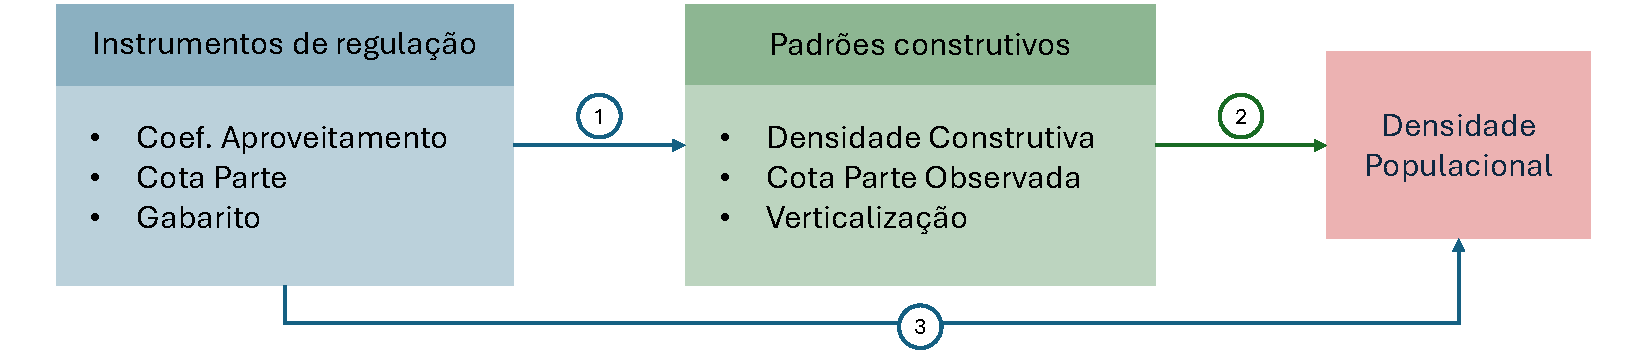
\includegraphics[width = \linewidth]{figuras/desenho_proposta.pdf}
    \label{fig:diagrama}
\end{figure}

\subsection*{A regulação foi capaz de influenciar os padrões construtivos na cidade da maneira esperada?} 

Através dos instrumentos apresentados na Seção \ref{sec:plano-diretor}, o PDE pretendia que o desenvolvimento imobiliário se concentrasse na Macrozona de Estruturação e Qualificação Urbana, em especial nos EETUs, que receberam um novo conjunto de regras. Em grande parte, essas mudanças permitiram um adensamento construtivo maior, verticalização ilimitada e impuseram uma densidade habitacional mínima. Todavia, como mencionado na Seção \ref{sec:motivacao}, a cidade é composta de diversos interesses, sendo o mercado imobiliário um agente central nesse aspecto. 

O mercado imobiliário, responsável por de fato construir novas habitacões, responde à regulação sempre buscando maximizar seu lucro. Como a regulação não criou incentivos e na verdade, apenas mudou permissões em cada região da cidade, não necessariamente o mercado imobiliário aceita o novo conjunto de regras como um convite para construir a tipologia que o PDE deseja ver nos EETUs. Dentro dos limites da legislação de CA entre 2 e 4, há muita liberdade para o mercado escolher o que construir. Ademais, sempre existe a opção de não construir nessas regiões, quando o benefício do maior potencial construtivo não é suficiente para compensar a taxação advinda da extrapolação do CA básico. 

\subsection*{Os padrões construtivos regulamentados e incentivados são de fato capazes de gerar a densidade esperada?} 

Em outras palavras, é possível afirmar que mais densidade construtiva, mais verticalização e mais densidade habitacional equivale a mais densidade populacional? Apesar de simples a pergunta, há certas nuances. Primeiramente, é importante identificar se os três componentes do padrão construtivo são importantes e qual apresenta maior relevância na determinação da densidade populacional. 

Caso a densidade construtiva seja um determinante para a densidade populacional, o instrumento do CA é importante. De maneira análoga, caso a densidade habitacional ou a verticalização se destaquem, a cota parte e o gabarito também são importantes. Nesse sentido, responder esta pergunta ajuda a identificar quais intrumentos analisados na pergunta 1 são mais importantes.

\subsection*{A regulação foi capaz de influenciar a densidade populacional na cidade?} 

O PDE propôs uma relação causal, ilustrada na Figura \ref{fig:diagrama}, que pressupõe que, se as duas primeiras condições forem atendidas, o aumento da densidade populacional será uma consequência direta. Ou seja, a terceira pergunta se tornaria desnecessária caso as duas primeiras se confirmassem.

Contudo, essa relação não é garantida, pois outros fatores também podem influenciar a densidade populacional, independentemente das regulamentações introduzidas. Assim, é essencial avaliar o efeito total da regulação sobre a densidade populacional, a fim de compreender o impacto completo e real das políticas implementadas.

\subsection*{Direcionamento no artigo}

No Capítulo \ref{chp:dados} serão apresentados os dados utilizado nas análises. No Capítulo \ref{chp:revisao} é feita uma breve revisão literária. No Capítulo \ref{chp:analise} será discutida a metodologia e resultados para cada uma das perguntas, na Seção \ref{sec:perg1}, \ref{sec:perg2} e \ref{sec:perg3}, respectivamente. No Capítulo \ref{chp:conclusao} serão trazidas as reflexões finais, na Seção \ref{sec:conclusao} o foco é nos principais resultados, e na \ref{sec:contribuicoes} é feita uma discussão com implicação mais direta no debate público. Por fim, nos Apêndices há discussões de detalhes importantes, mas que tangenciam a narrativa do trabalho.

Os códigos utilizados para gerar os resultados apresentados estão disponíveis de maneira pública para verificação, replicação ou utilização para outros fins, contato que este trabalho seja citado de maneira adequada\footnote{O código pode ser acessado na página do GitHub \href{https://github.com/gustavo-tm}{neste link.}}.


\chapter{Revisão Literária}
\label{chp:revisao}

\section{Importância da regulamentação}

Na literatura microeconômica há diversos modelos que tentam compreender as dinâmicas econômicas da cidade, analisando como as forças de mercado agem na ausência da regulação. Utilizando premissas formais e provas matemáticas, é possível resolver os modelos para algumas variáveis endógenas, como preço por metro quadrado na cidade, uso do solo, densidade populacional, entre outros. O que geralmente há de comum entre estes modelos, é que se o mercado receber um tratamento \textit{laissez-faire}, se observará um maior adensamento no centro, onde há oferta de emprego. Quando há múltiplos centros, ou pontos de transporte público de alta capacidade, também há maior adensamento no entorno deles \cite{papageorgiou2012essay, fujita1989urban}.


Isso acontece porque o adensamento traz diversos benefícios econômicos. A aglomeração tecnológica $(i)$ aumenta a produtividade dos trabalhadores, na medida em que os empregos são mais concentrados e há ``transbordamento'' de conhecimento entre as firmas da região. Além disso, uma oferta maior e mais diversa de trabalho, causa maior competitividade e eficiência na escolha da pessoa certa para cada cargo. Aglomerações pecuniárias $(ii)$ reduzem os custos das firmas, sem alterar sua produtividade. Com maior demanda por serviços como segurança, limpeza, contratação e advocacia, estes mercados se desenvolvem, tornam-se mais competitivos, eficientes e baratos. Inclusive, há serviços especializados de nicho, que podem estar disponíveis e acessíveis apenas em grandes centros urbanos. Aglomeração de varejo $(iii)$ traz ganhos para os consumidores e comerciantes. Quando o comércio está aglomerado, o consumidor pode escolher entre mais opções e se desloca menos entre seus destinos caso queria comprar mais de um item. Dessa forma, os consumidores ganham e os comerciantes também, visto que com mais consumidores e maior fluxo, maiores as vendas. Por fim, o custo de transporte $(iv)$ é um dos fatores que mais mudam quando há densidade. A redução do custo de transporte, que pode ser considerada uma economia de aglomeração pecuniária, acontece não apenas para os trabalhadores, que se deslocam menos às oportunidades de emprego, mas também às firmas que gastam menos transportando seus bens e serviços \cite{brueckner2011lectures}.

Entretanto, ao introduzir falhas de mercado nesses modelos, a organização da cidade na ausência de regulamentação pode estar associada cenários não desejáveis. Muitas vezes estas falhas de mercado encadeam uma expansão da mancha urbana, com implicações negativas no meio ambiente, além da perda dos benefícios da aglomeração. Um exemplo de falha de mercado está relacionada ao tráfego de carros. Este meio individual diminui os custos de transporte para longas distâncias, possibilitando que os cidadãos habitem residências mais distantes de seus destinos. Todavia, além de causar uma expansão da mancha urbana, introduzir risco de acidentes e emitir poluentes, cada carro a mais que está na rua torna a viagem de todas as outras pessoas um pouco mais lenta. Apesar desses malefícios serem negligenciáveis nas escolhas individuais de utilizar ou não o carro, ou seja, um indivíduo racional não vai deixar de usar o carro, em uma cidade com milhões de habitantes, o custo individual negligenciado de cada carro se soma, de forma a ter um impacto significativo para a sociedade.

Nesse sentido, o governo poderia intervir, de forma a corrigir estas falhas de mercado, por exemplo, introduzindo um pedágio urbano. Dessa forma, seriam internalizadas as externalidades negativas dessa escolha individual de usar o carro. Com o dinheiro coletado desse imposto, poderiam ser compensados os danos causados, através de investimentos públicos. Entretanto, tal medida é difícil de ser implementada, levando os tomadores de decisão a tomar outro caminho no combate às externalidades. Regular os padrões construtivos, pode ser uma forma alternativa de lidar com o problema, impedindo que as externalidades aconteçam. Nessa frente, o CA é o instrumento mais bem estabelecido na literatura do urbanismo para regular o padrão construtivos em cidades modernas nos Estados Unidos, Canadá, Alemanha, França, etc.

Caso o CA máximo regulado seja maior do que o mercado demanda, o CA observado será inferior ao limite, ou seja, a regulação não impacta essa região diretamente. Nas regiões em que a demanda por habitação é maior do que o permitido, parte da demanda precisam ser remanejada terriorialmente, para que o limite não seja ultrapassado. A ideia do PDE é limitar o adensamento nas regiões periféricas, direcionando o adensamento para as regiões centrais. Entretanto, caso o excesso de demanda esteja em uma área central, haverá um espraiamento para as periferias, causando o efeito contrário do estipulado. Na Figura \ref{fig:FAR} é possível observar um exemplo de CA máximo na cidade como um todo e a demanda por habitação excedente no centro, que com o limite máximo no CA, se dispersa em territórios mais distantes.

\begin{figure}[h]
    \caption{Impacto da regulação no CA da cidade}
    \centering
    \begin{subfigure}{.6\linewidth}
        \begin{tikzpicture}

    \begin{axis}[standard,
        xtick={0},
        ytick={.5},
        xticklabels = {},
        yticklabels = {$FAR_{reg}$},
        samples=100,
        xlabel={Distance to center ($x$)},
        ylabel={FAR},
        xmin=0,xmax=2,
        ymin=.2,ymax=1,
        y label style={anchor=east},
        x label style={anchor=north},
        clip=false
    ]
    
\addplot[domain={0:2}]{.8*e^(-.9*x)+.1} node[pos=1] (point1) {};
\node [right] at (point1) {\textit{laissez-faire}};

\addplot[domain={(ln(4.8)/1.3):2}]{1.2*e^(-1.3*x)+.25} node[pos=1] (point2) {};
\node [right] at (point2) {regulado};

\addplot[domain={0:(ln(4.8)/1.3)}]{.5};

\addplot[black, dashed] coordinates {((ln(4.8)/1.3),0) ((ln(4.8)/1.3),.5)};

\end{axis}
\end{tikzpicture}
    \end{subfigure}
    \label{fig:FAR}
\end{figure}

Portanto, caso o planejador central identifique incorretamente a demanda de mercado em cada região da cidade, é possível que a demanda reprimida encadeie um processo de expansão da mancha urbana e todas as externalidades negativas discutidas anteriormente. Nesse sentido o CA, apesar de ser uma ferramenta poderosa no arsenal do planejador urbano, ela também é perigosa, visto que pode levar a efeitos adversos. 

\section{Evidências do PDE de 2014}


\chapter{Dados}
\label{chp:dados}

\section{Padrões Construtivos}
\label{sec:dadosIPTU}

Em relação aos dados sobre os empreendimentos imobiliários, a base de dados escolhida foi do IPTU. Para os fins deste artigo, ela é a mais completa, visto que não representa um fluxo de novos imóveis construídos todos os anos como a base da Embraesp, mas apresenta um estoque imobiliário de tudo que já foi construído de moradia formal na cidade. Dito isso, estão cadastrados os 3.096.719 números únicos de contribuintes, que, segundo a definição da documentação dos dados no GeoSampa, ``A cada imóvel urbano corresponderá um número de inscrição no Cadastro Imobiliário Fiscal, entendendo-se como imóvel: I - a área de terreno, construído ou não, definida em matrícula do competente Serviço de Registro de Imóveis ou em transcrições ainda vigente''. Os únicos dados que não constam nessa base são relativos a lotes irregulares ou não registrados.

Entre os dados disponíveis do IPTU, se destacam a área do terreno, a área construída, a área ocupada, o tipo de uso e o número de pavimentos do empreendimento. Logo, com estes dados é possível identificar os padrões construtivos na cidade, mantendo os cálculos os mais fiés possível à forma como são calculados pela regulação. A densidade construída, por exemplo, é definida pelo CA observado na construção -- não é considerando nesta análise o CA regulado da região. 

\begin{figure}[h]
    \centering
    \caption{Distribuição do padrão construtivo em cada lote residencial de São Paulo}
    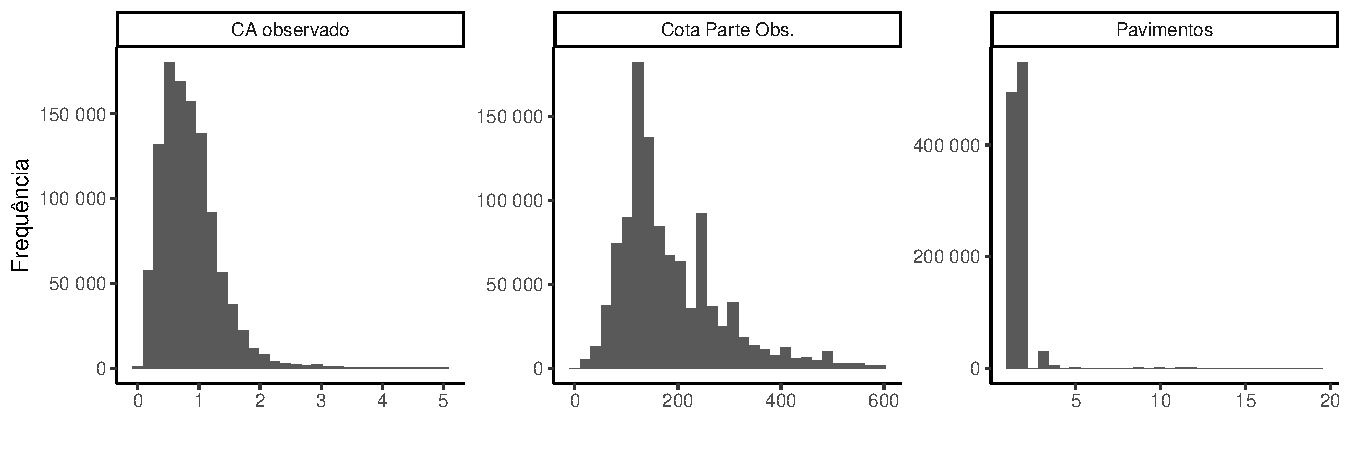
\includegraphics[width = \linewidth]{figuras/indicadores.pdf}
    \label{fig:histogramas}
\end{figure}

De fato, ao observar os indicadores na Figura \ref{fig:histogramas}, é possível notar que o perfil habitacional de São Paulo é bastante horizontal. É surpreendente que 95\% dos lotes residenciais em São Paulo apresentam 2 ou menos pavimentos. Ainda, a mediana do CA observado é 0,8, o que indica que em mais da metade dos lotes da cidade foi construído menos do que a área do terreno. Ainda, a cota parte observada mediana dos lotes da cidade é de 155$m^2$, o que representa um uso do terreno para poucas unidades habitacionais em média -- a cota parte observada mediana é aproximadamente 8 vezes maior do que a cota parte máxima nos EETUs. Na Figura \ref{fig:indicadores-tempo} do Apêndice \ref{appendix:figuras} é possível observar a evolução dos padrões construtivos no tempo e na Figura \ref{fig:area_construida} está a distribuição da área construída dedicada a cada tipo de uso e perfil de densidade.

\section{Regulação}
\label{sec:dadosPDE}

Os dados da regulação são disponibilizados também de maneira pública no site da prefeitura junto ao PDE, mas pode também ser acessado pelo GeoSampa. O principal dado utilizado foi das áreas de influência dos ativadores de eixo, para que cada lote pudesse ser classificado como dentro ou fora da região de EETU.

\section{Densidade populacional}
\label{sec:dadosCenso}

Os dados de densidade populacional, são produzidos pelo Censo demográfico do IBGE, que ocorre a cada 10 anos. O censo de 2020 se atrasou para 2022 por conta da pandemia e os dados começaram a ser divulgados em 2024. Até o momento, o que foi disponibilizado de maneira pública é a malha preliminar do censo. Considerando que o PDE entrou em vigor em 2014, foi utilizado o censo de 2010 como um período pré PDE e o censo de 2022 como periodo pós. Segundo o levantamento de 2022, a atual população do município de SP se encontra em 11.451.999 de habitantes, dividios em 4.996.529 de domicílios, dos quais apenas 4.316.336 estão ocupados. Na Figura \ref{fig:populacao} do Apêndice \ref{appendix:figuras} é possível observar quais são as áreas mais densas da cidade. 


A unidade de observação do censo mais próxima de microdados que pode ser georreferenciada é o setor censitário\footnote{Para estar em conformidade com a Lei Geral de Proteção de Dados (LGPD), é importante proteger a anonimidade dos entrevistados, então deve haver algum tipo de agregação geográfica.}. Os limites dos setores são construídos de forma que o agente de coleta do censo consiga cobrir o setor inteiro, minimizando os erros de medição e otimizando o processo. A metodologia para a delimitação dos setores censitários leva em consideração diversos fatores, como elementos na paisagem que se constituam em barreiras naturais ou artificiais e dificultam o trabalho do agente, pontos de referência estáveis e de fácil identificação no terreno, limites das estruturas territoriais como bairros e quadras, entre outros \cite{IBGE2024}. Um fator determinante para o tamanho do setor censitário é o número de domicílios a serem entrevistados, que em áreas urbanizadas deve estar entre 250 e 400 para os mais densos e entre 150 e 250 para os menos densos.

\section{Cruzamento dos dados}
\label{sec:dadosCruz}

Parte da dificuldade de discutir os temas urbanos com dados é a complexidade de trabalhar com eles. Como é possível observar na Tabela \ref{tab:dados}, cada dado apresenta um nível de observação e frequência diferente. Portanto, sempre é necessário que haja alguma agregação territorial ou temporal para que a análise seja possível. Como comentado anteriormente, a metodologia de processamento de dados utilizada neste artigo está disponível em um repositório público.

\begin{table}[h!]
    \centering
    \caption{Information about each database}

    {\small
    \begin{tabular}{>{\raggedright\arraybackslash}p{0.125\linewidth} >{\raggedright\arraybackslash}p{0.50\linewidth} >{\centering\arraybackslash}p{0.125\linewidth} >{\raggedright\arraybackslash}p{0.15\linewidth}}
        % \toprule
        \textbf{Data} & \textbf{Source} & \textbf{Frequency} & \textbf{Scale} \\
        \midrule
        Census & Brazilian Institute of Geography and Statistics (IBGE) & Decennial & Census tract \\
        Property Tax (IPTU) & Property Tax and Maintenance Registry maintained by the Municipal Department of Finance (DECAD) of São Paulo's City Hall & Annual & Taxpayer \\
        Plots & Fiscal Real Estate Registry of the Municipal Department of Finance & Annual & Plot \\
        Regulation & Department of Urbanism and Licensing (SMUL) & 2014 & Zone perimeter \\
        \bottomrule
    \end{tabular}
    }
    \label{tab:datasets}
\end{table}


Os dados do IPTU não são georreferenciados, então desacompanhados de outros dados não é possível cruzá-los com os do Censo. O que possibilita fazer essa junção é que o número único de contribuinte do IPTU, também é o código do Setor, Quadra e Lote (SQL) que o empreendimento se encontra. Nesse sentido, é possível decompor o SQL e cruzar com as bases de lotes, que contêm a geometria de cada  um dos 1.677.980 lotes da cidade. O que explica a diferença entre o número de lotes e número de números dos contribuintes são os lotes que contém um condomínio, que pode haver diversos números únicos de contribuintes em apenas um lote. Nos dados de IPTU, há 1.314.353 contribuintes em lotes com apenas uma unidade habitacional e 33.129 condomínios, que contêm 1.782.366 unidades. Ao cruzar o SQL do IPTU com a base de lotes, 44.319 contribuintes não encontram um par na outra base, o que representa uma perda de 1,67\% das unidades. 

Os dados da regulação não são codificados com o SQL, mas podem ser cruzados geograficamente. O perímetro de zona é um limite parecido com a quadra, que pode ser recortada em alguns casos. Para determinar quais áreas são de EETUs, os perímetros de zona foram unidos, de forma a considerar todo o espaço interior e um contorno das regiões de EETU foi criada. O mapa com o resultado pode ser visto no Apêndica \ref{appendix:figuras}, Figura \ref{fig:eixos}. 

Como o perímetro de zona é bastante aderente à estrutura das quadras, a classificação dos lotes em estar dentro ou fora da região de eixo é direta. Por outro lado, os setores censitários seguem uma estrutura completamente diferente. Há vezes que um setor censitário contém diversos lotes, mas é possível que um lote contenha também mais de um setor censitário. Para fins práticos, os dados do IPTU, censo e regulação foram cruzados geograficamente. Uma discussão com maior detalhamento pode ser consultada no Apêndice \ref{appendix:cruzamento}.

Os setores censitários são uma partição\footnote{Uma partição é uma divisão que ocupa o espaço por completo, sem que haja intersecção entre os elementos} do espaço da cidade de São Paulo, o que implica que a área do setor censitário é composta não apenas pelos lotes, mas também por trechos que contém ruas, parques, usos não residenciais, entre outros fatores. Na Figura \ref{fig:area-setor} é possível identificar que apenas um terço da área do setor censitário é dedicado ao uso residencial. Além disso, no raio de 1km dos eixos, aproximadamente 4\% dos empreendimentos residenciais foram construídos após 2014\footnote{Este valor está superestimado, visto que grande parte dos prédios que ficaram prontos entre 2014 a 2017 foram aprovados durante a vigência do PDE de 2002}, que foi o período em que o PDE entrou em vigor. 
 
\begin{figure}[h]
    \centering
    \caption{Dedicação do espaço do setor censitário para cada uso em um raio de 1km dos eixos}
    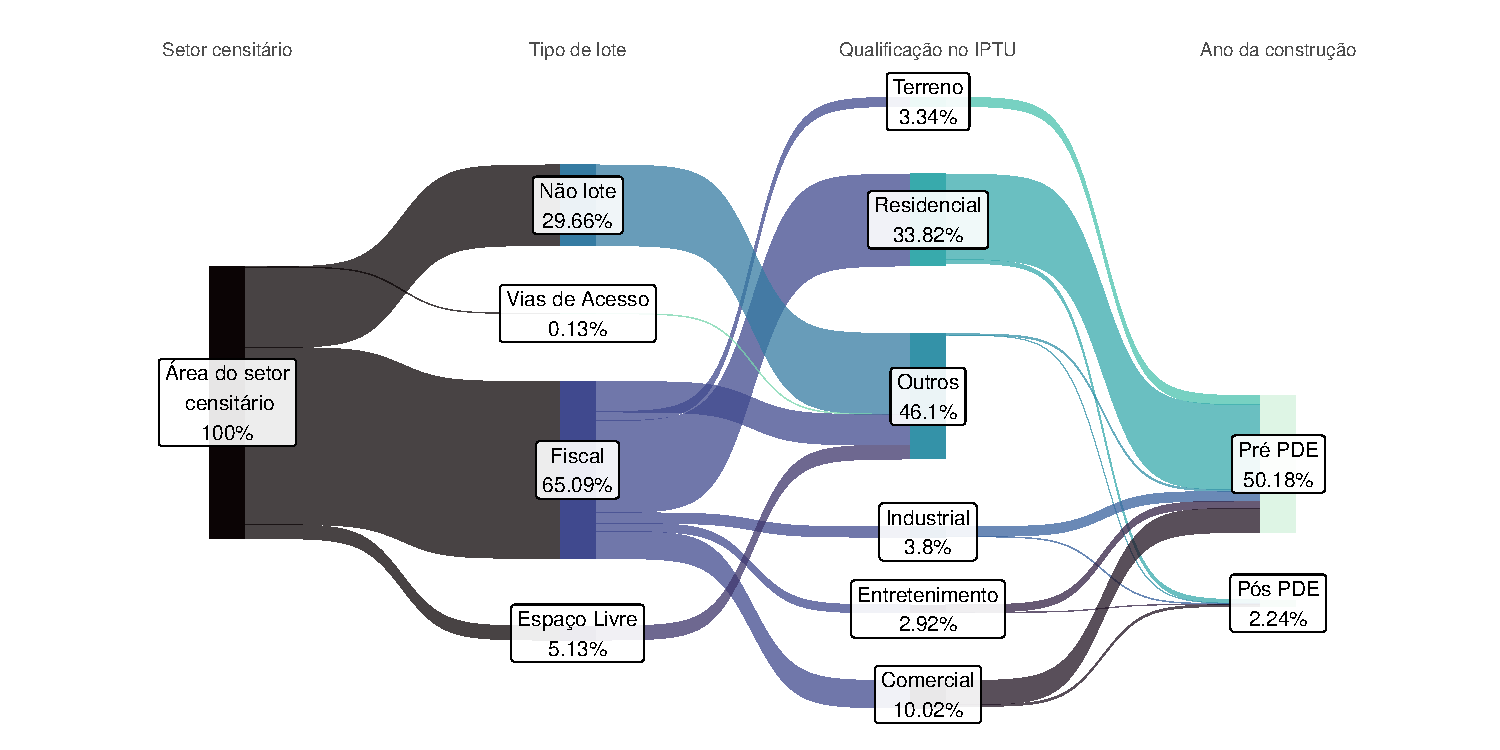
\includegraphics[width = \linewidth]{figuras/area_setor.pdf}
    \label{fig:area-setor}
\end{figure}

\chapter{Metodologia e Resultados}
\label{chp:analise}

Como comentado na Seção \ref{sec:problema}, há três perguntas a ser respondidas, que podem ser visualizadas no diagram da Figura \ref{fig:diagrama}. Nas seções a seguir, cada uma das perguntas será respondida através da análise quantitativa dos dados apresentados.


\section{Do padrão construtivo à densidade populacional}
\label{sec:perg1}


O objetivo desta seção é responder: \textbf{Os padrões construtivos regulamentados e incentivados são de fato capazes de gerar a densidade esperada?} Para tanto, foram considerados os dados do Censo de 2022 e os do IPTU do mesmo ano. Para esta seção, a regulação de cada região da cidade não é importante, visto que o foco é em identificar qual a relação entre a densidade construtiva, densidade habitacional e pavimentos com a densidade populacional. Esta relação não é modificada pelo PDE. A influência sobre estes três componentes do padrão construtivo por parte do PDE se dá através do CA, cota parte e gabarito, respectivamente. Dessa forma, validar a importância desses padrões construtivos significa validar também os instrumentos de regulação.

Para inferir a relação entre as 3 variáveis e a densidade populacional, foram adotadas duas abordagens. A primeira foi de utilizar uma regressão linear. A principal limitação dessa abordagem é que a forma funcional da regressão não está fundamentada economicamente, o que a torna sujeita a problemas de endogeneidade, e, portanto, enfraquece a validade da inferência. A abordagem alternativa, de árvores de regressão, transita do universo da econometria para o universo do \textit{machine learning}. 

O primeiro passo para implementar estas metodologias consiste em combinar as bases de dados em um nível de observação único. Para manter os dados na escala mais desagregada possível, os dados poderiam ser agregados ao nível do setor censitário. Porém, como foi discutido na Seção \ref{sec:dadosCenso}, o tamanho do setor censitário depende diretamente tanto da população que o habita, quanto de sua densidade, o que traria viés para a regressão\footnote{Neste caso, a densidade populacional depende da área do setor censitário, que não pode ser omitida da regressão. Entretanto, se for utilizada como um regressor, apresentará uma relação de simultaneidade com a variável dependente, já que quanto mais densa uma região é, menor será sua área. Sendo assim, seria necessário fazer uma estimação por equações simultâneas, trazendo complexidade para a identificação, já que não há variáveis exógenas suficientes para recuperar os parâmetros de interesse}. Desse modo, o mapa da cidade foi recortado em um \textit{raster} (quadriculado) com células de 800m de largura. Os detalhes mais técnicos podem ser encontrados no Apêndice \ref{appendix:cruzamento}. Por fim, foram filtrados apenas as células do raster que tivessem um grau baixo de informalidade. Para mais detalhes sobre a informalidade, consultar o Apêndice \ref{appendix:informalidade}. 


\section{Da regulação ao padrão construtivo}
\label{sec:perg2}

\section{Da regulação à densidade populacional}
\label{sec:perg3}

\chapter{Conclusão}
\label{chp:conclusao}

\section{Resultados principais}
\label{sec:conclusao}

\section{Contribuições para o debate público}
\label{sec:contribuicoes}

